\section{Hardened 1st-order Masked Sbox for RECTANGLE}\label{sec:rectangle}
We have discussed the ILA-breaching effects in Section~\ref{sec:ila_effects} and integrated these observations in the ASCOLD tool,  described in Section~\ref{sec:tool}. The current Section builds up on these advances by putting forward a ``hardened", 1st-order masked, ISW-based RECTANGLE Sbox. The desired aim is to produce an assembly-based, lightweight Sbox implementation that is secure against 1st-order, univariate attacks, hence forcing the attacker to resort to 2nd-order and/or multivariate techniques. 

Our implementation opts for a bitsliced~\cite{DBLP:conf/fse/DaemenGV93,DBLP:conf/fse/Biham97a} representation, due to both the bitsliced structure of RECTANGLE and to the $GF(2)$-oriented nature of the ISW countermeasure. We employ a bitslicing factor of 2, i.e. we exploit the 8-bit AVR architecture in order to process two 4-bit Sboxes in parallel (nibble-slicing). The Sbox is decomposed into $GF(2)$ operations which can be accelerated by via SIMD-like, 8-bit assembly instructions. The decomposition suggested by Zhang et al.~\cite{DBLP:journals/chinaf/ZhangBLR0V15} is optimal w.r.t. $GF(2)$ multiplicative complexity, since Grosso et al.~\cite{DBLP:conf/fse/GrossoLSV14} established that the minimum number of non-linear operations required by 4x4 Sboxes is 4. 

In order to ``harden" the Sbox, we use the solutions suggested in Section~\ref{sec:ila_effects} and follow two approaches: efficient and conservative. In the \emph{efficient} approach, after processing any share, we clear the registers on a need-to basis and insert dummy \texttt{ld} instructions to avoid overwrite and remnant effects. We avoid neighbouring leakage effects by always storing the shares in SRAM, i.e. the register file contains only the shares used by the current instruction. In the \emph{conservative} approach, we perform all the afore-mentioned clearing techniques. In addition, we insert dummy \texttt{st} instructions and perform thorough register/memory clearing. Both efficient and conservative approaches are applied to every single instruction of the implementation, i.e. the cost is linear w.r.t. the number of instructions that manipulate masked shares. The resulting computational overhead is significant: the efficient ``hardened" Sbox implementation runs in 993 clock cycles, i.e. almost 12 times slower compared to the ``naive" 1st-order, ISW-based RECTANGLE Sbox, which runs in $87$ clock cycles. The conservative ``hardened" Sbox implementation requires 1319 clock cycles, i.e. it is 15 times slower. Table~\ref{cc_table} contains a comparison between ``naive" 1st-order, ``naive" 2nd-order and efficient/conservative ``hardened" 1st-order bitsliced implementations of the RECTANGLE Sbox in AVR assembly.
\begin{table}[H]
\centering
\caption{Masked Sbox comparison in ATMega163}
\label{cc_table}
\begin{tabular}{ |l|l|l|l|l|}
\hline
\textbf{Order $\mathbf{d}$} & \textbf{Hardened} & \textbf{Latency (cc) }& \pbox{20cm}{ \textbf{Throughput} \\ \textbf{(bits/cc $\mathbf{*10^{-3}}$)} }& \textbf{RNG (bytes)} \\ \hline \hline 
Unprotected  & no & 32 & 250 & 0 \\ \hline
1st order      &   no & 87 & 91 &  4\\ \hline
 1st order      &   yes (eff.)& 993 & 8 & 4\\ \hline
 1st order      &   yes (cons.) & 1319 & 6 & 4\\ \hline
 2nd order     &   no  & 775 & 10 & 12\\ \hline
\end{tabular}
\end{table}

Using the 1st-order, random vs. fixed t-test, we evaluate the efficient and conservative ``hardened" 1st-order Sboxes, as well as the ``naive" 1st-order Sbox. Using a $25$k random vs. $25$k fixed t-test does not yield any statistically significant leakage in the efficient ``hardened" version (Figure~\ref{hardbox_eff}). However, wenote that a $50$k random vs. $50$k fixed t-test is able to detect leakage, i.e. trying to reduce the cost of enforcing ILA can have a detrimental effect on security. For the conservative ``hardened" Sbox, a 100k random vs. 100k fixed t-test does not detect any leakage (Figure~\ref{hardbox_cons}). Note that a \emph{2nd-order} $25$k random vs. $25$k fixed t-test on a chosen sample window is able to detect leakage. Therefore, we conclude that for the given device, the informativeness of 1st-order attacks is substantially limited and a 2nd-order attack is the preferable adversarial strategy (Figure~\ref{t_order2}). Naturally, the ``naive" 1st-order version rejects the null hypothesis (Figure~\ref{softbox}) due to the ILA-breaching effects and the 1st-order leakage can be easily exploited.
\begin{figure}[H]

 \begin{subfigure}[b]{0.40\textwidth}
        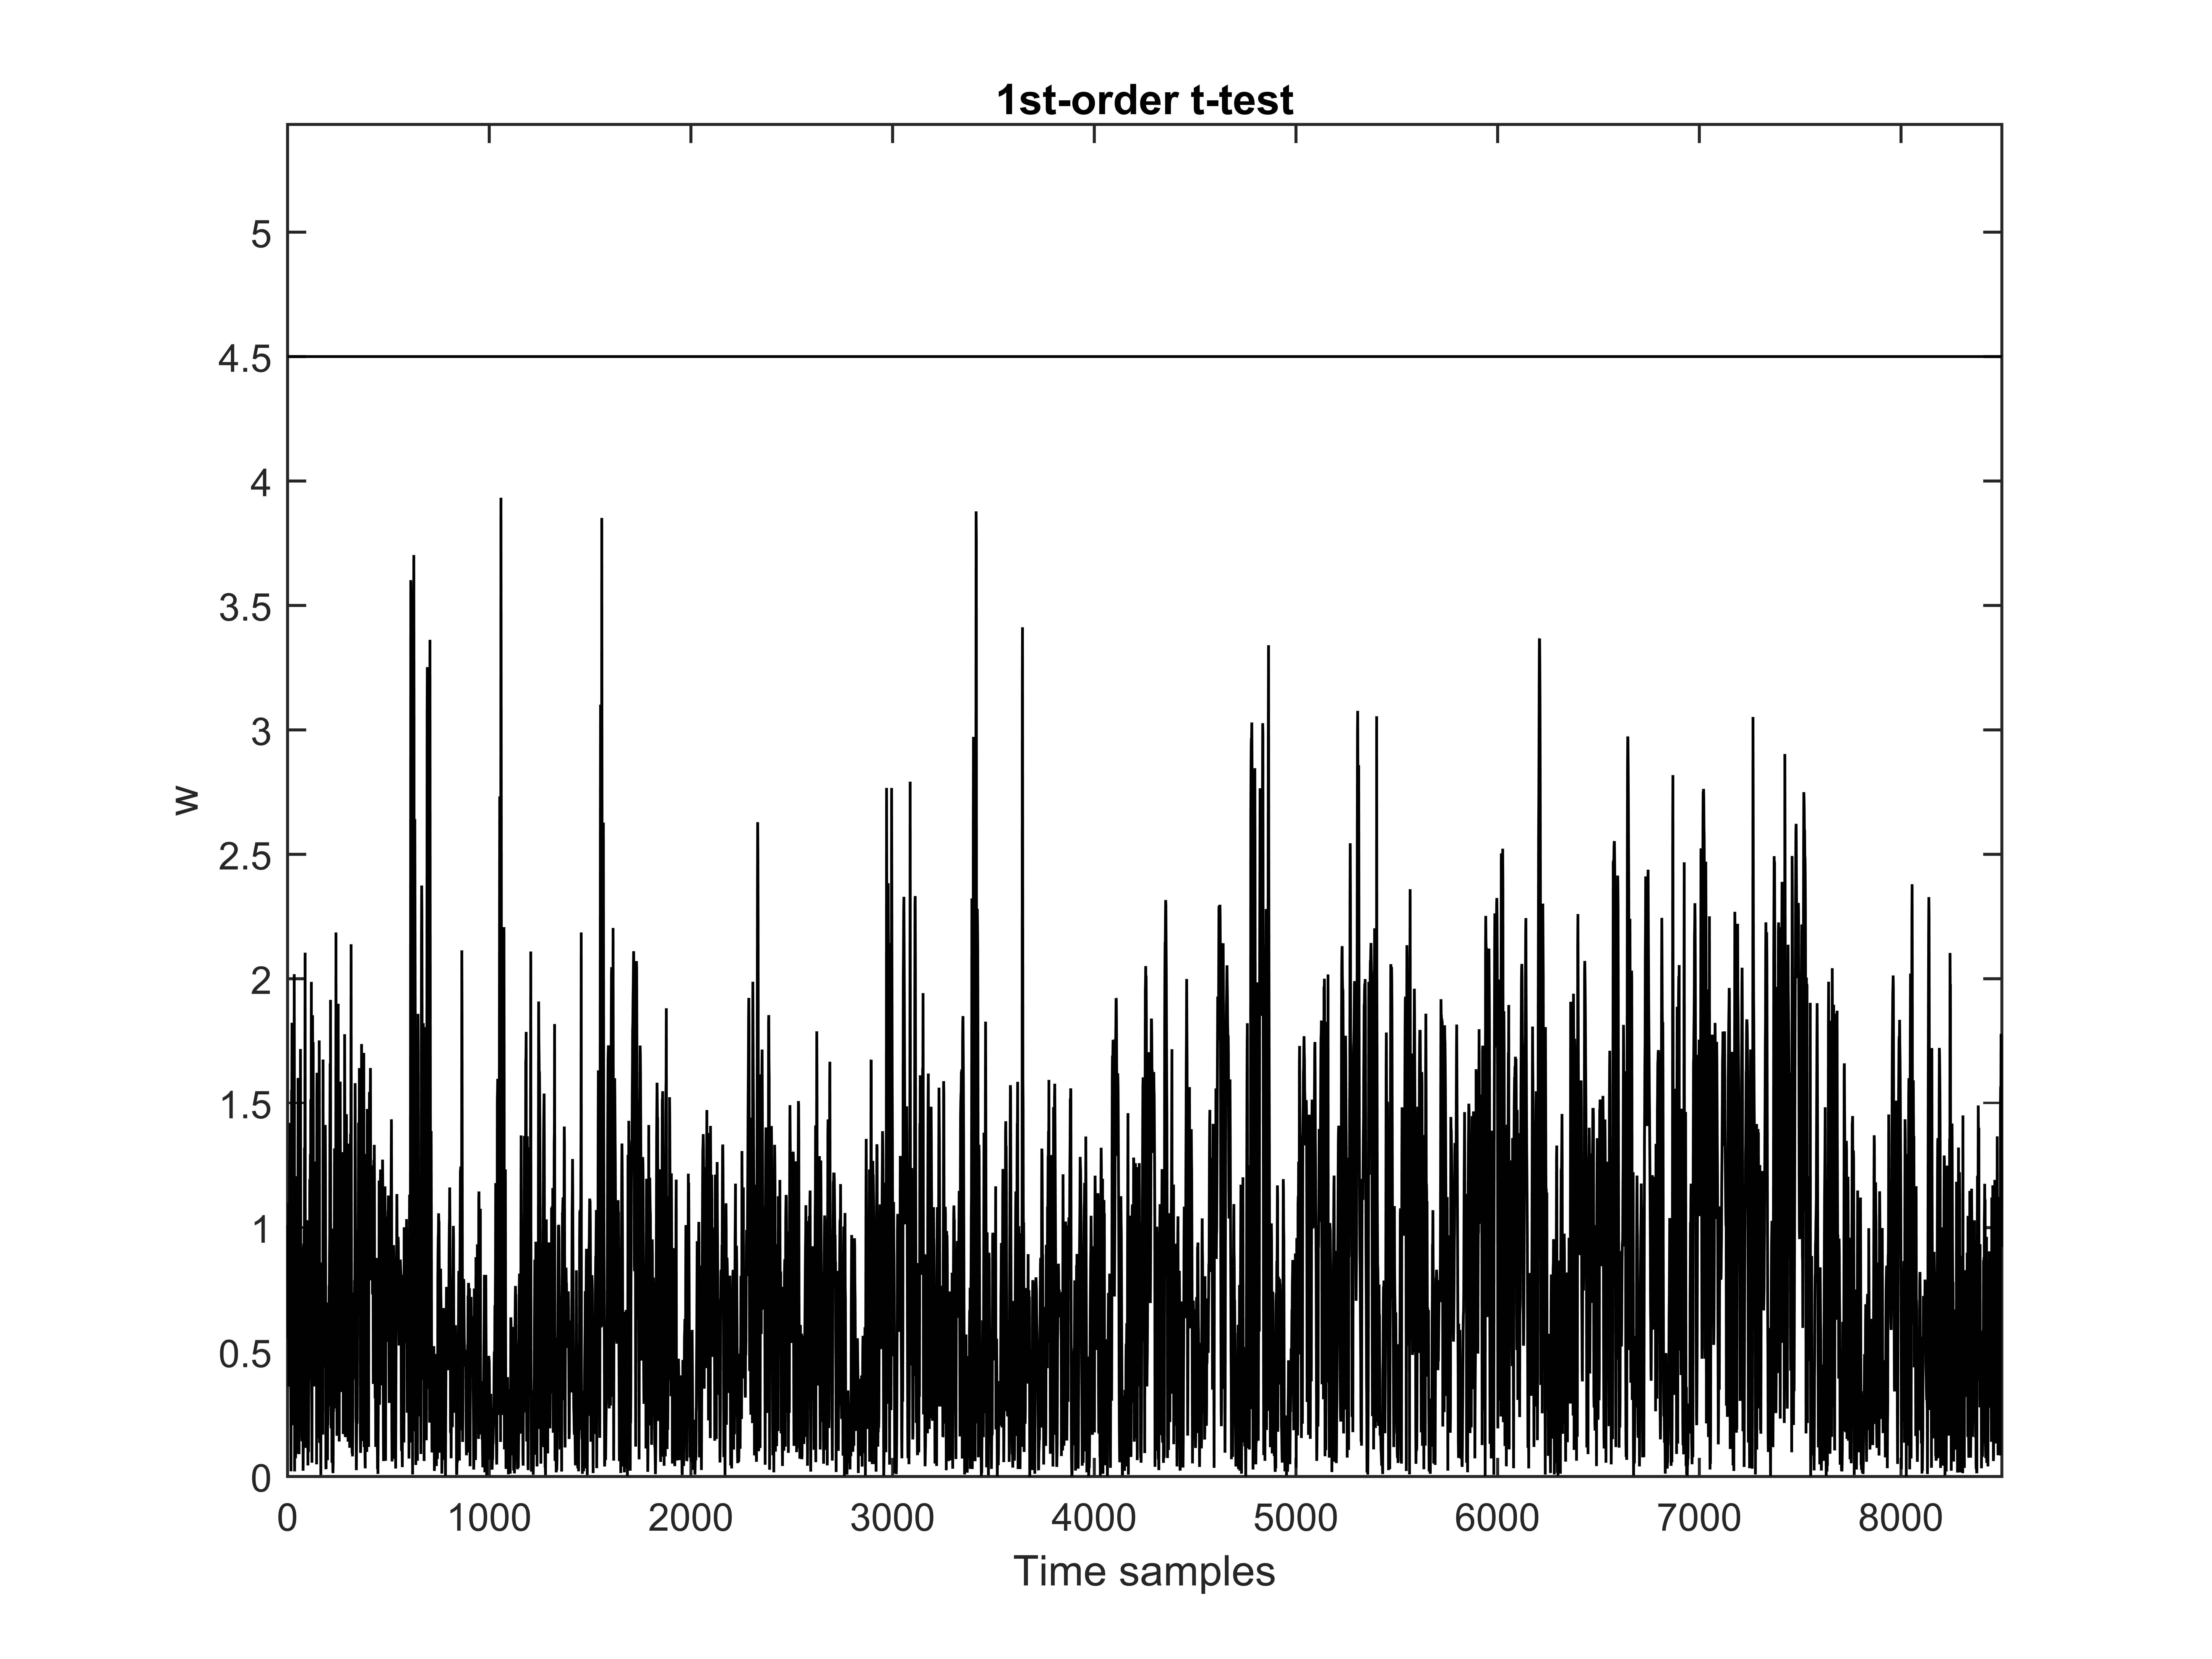
\includegraphics[width=\textwidth]{{fig/hardbox_eff.png}}

        \caption{\scriptsize{Efficient hardened Sbox, 1st-order t-test, 25k random vs. 25k fixed.}}
\label{hardbox_eff}
    \end{subfigure}  \hspace{15px}
 \begin{subfigure}[b]{0.40\textwidth}
        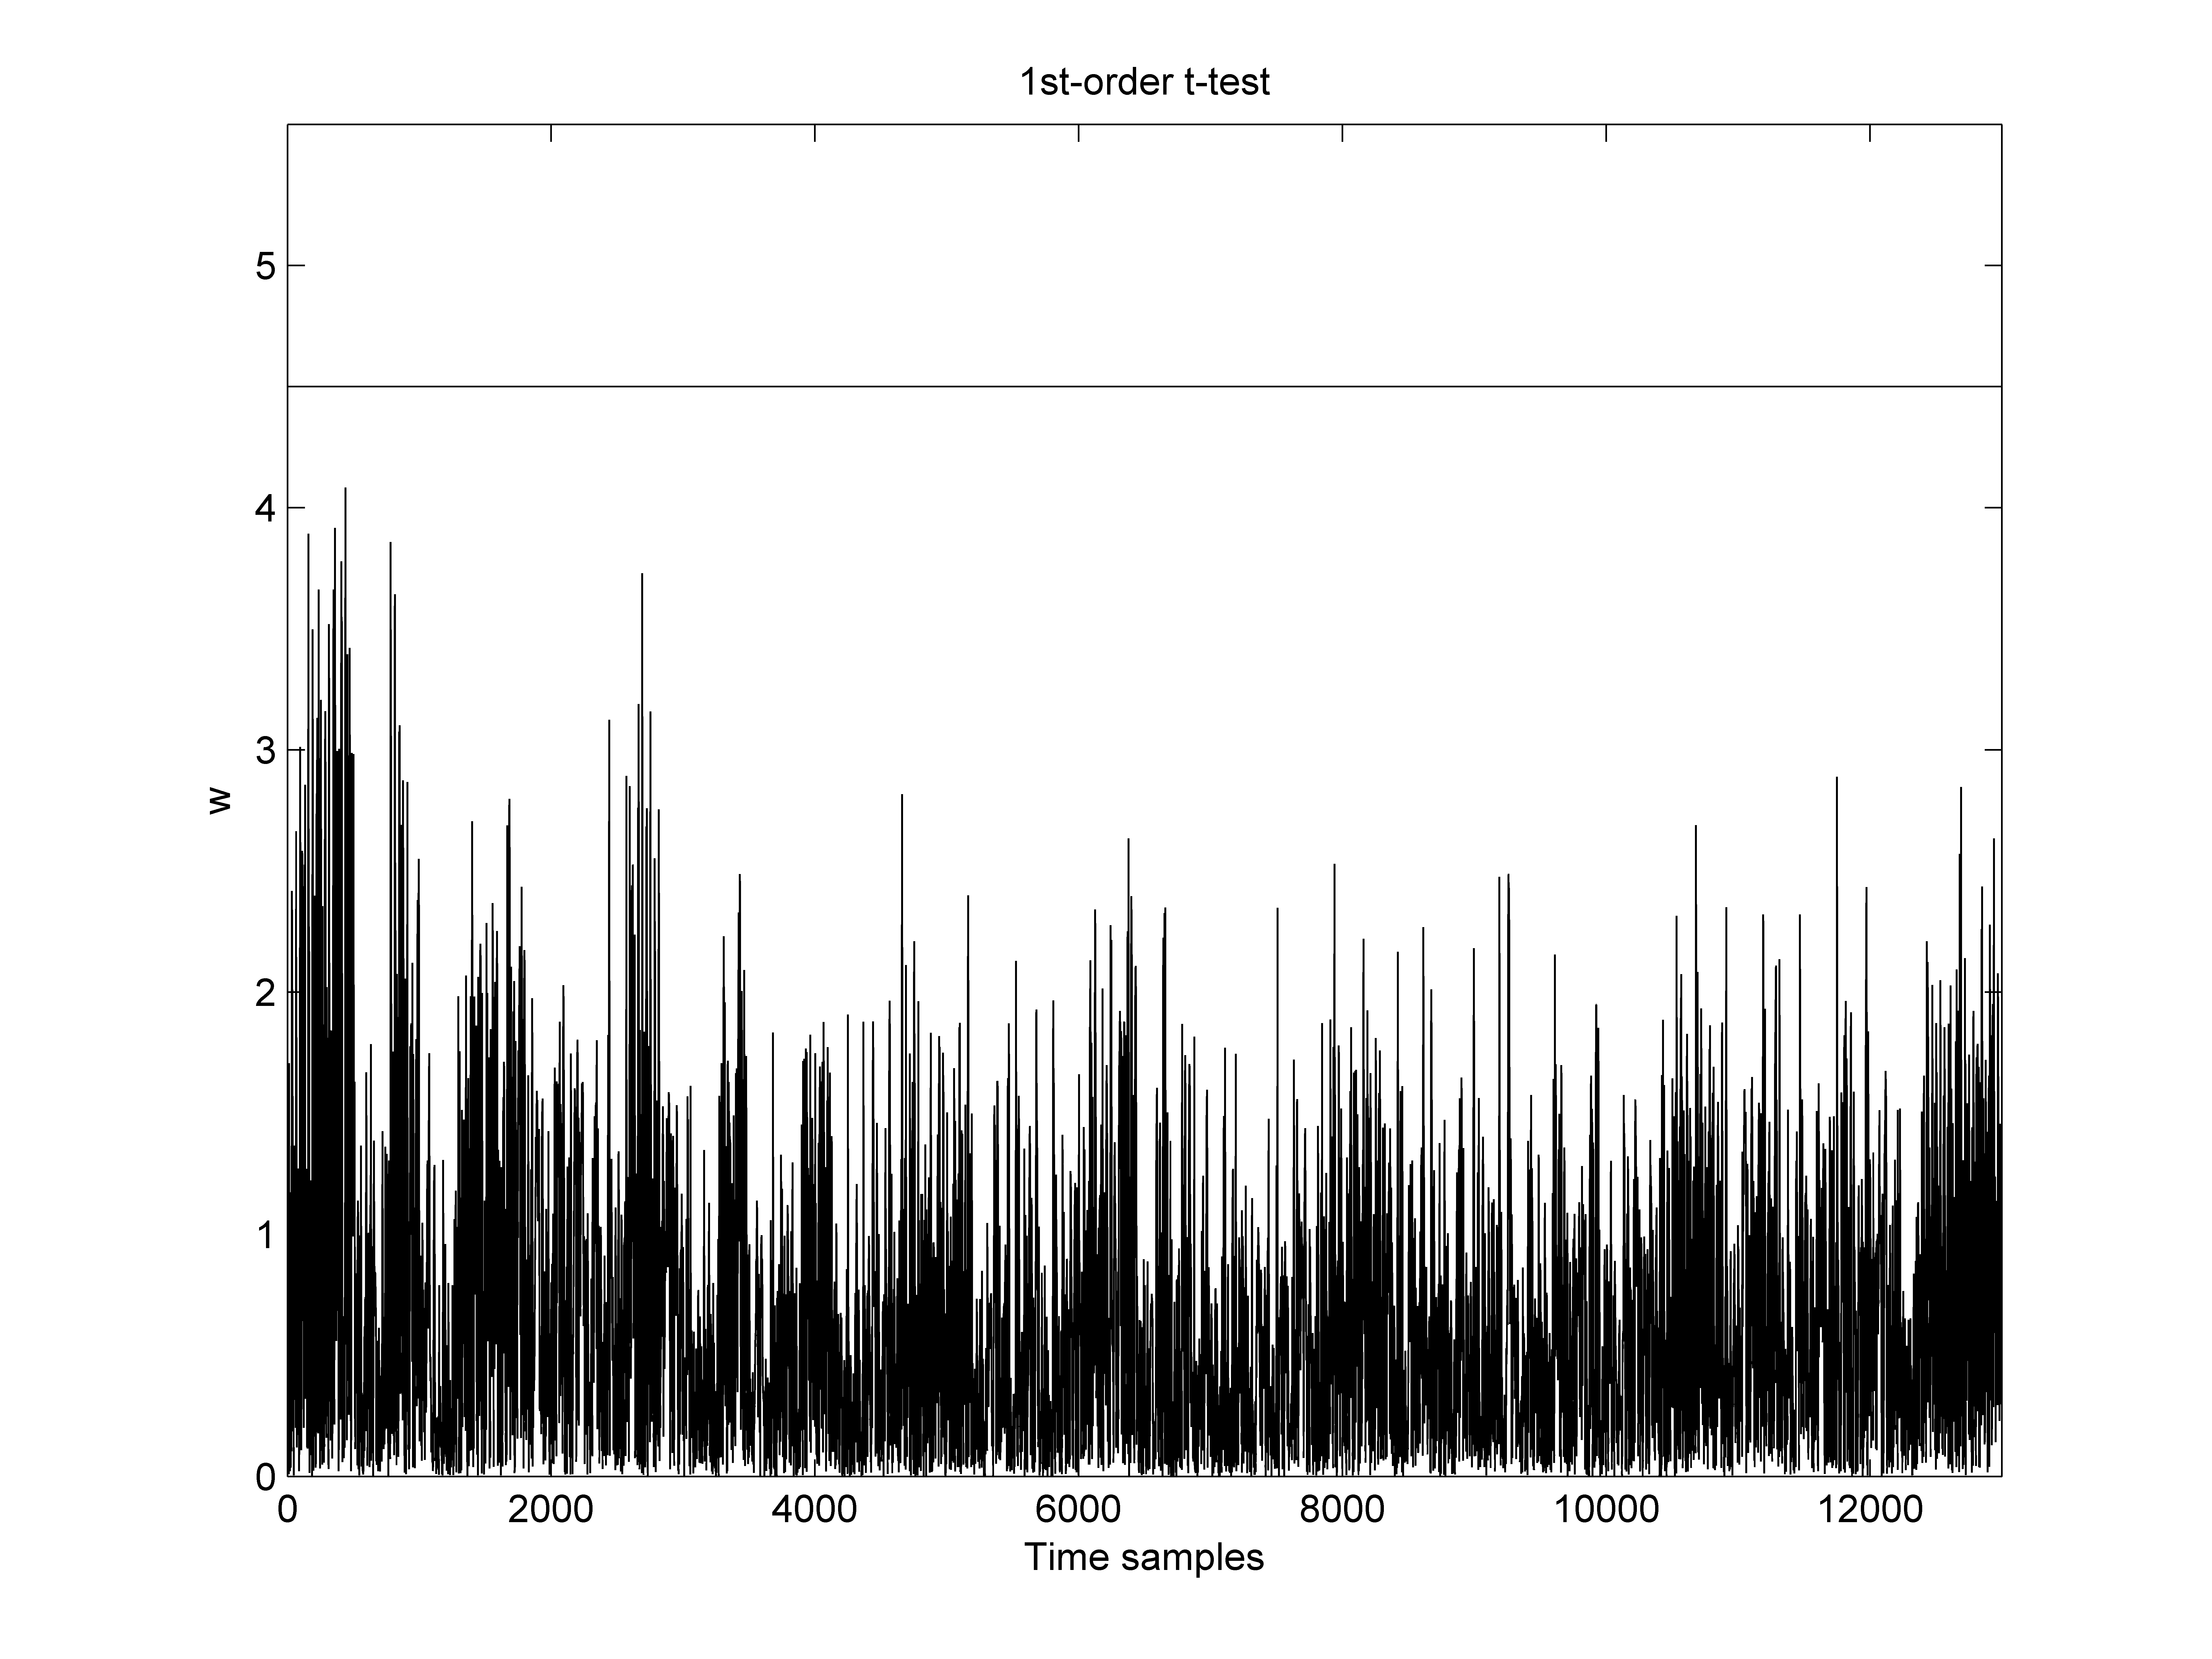
\includegraphics[width=\textwidth]{{fig/hardbox_cons.png}}

        \caption{\scriptsize{Conservative hardened Sbox, 1st-order t-test, 100k random vs. 100k fixed.}}
\label{hardbox_cons}
    \end{subfigure}

\begin{subfigure}[b]{0.40\textwidth}
        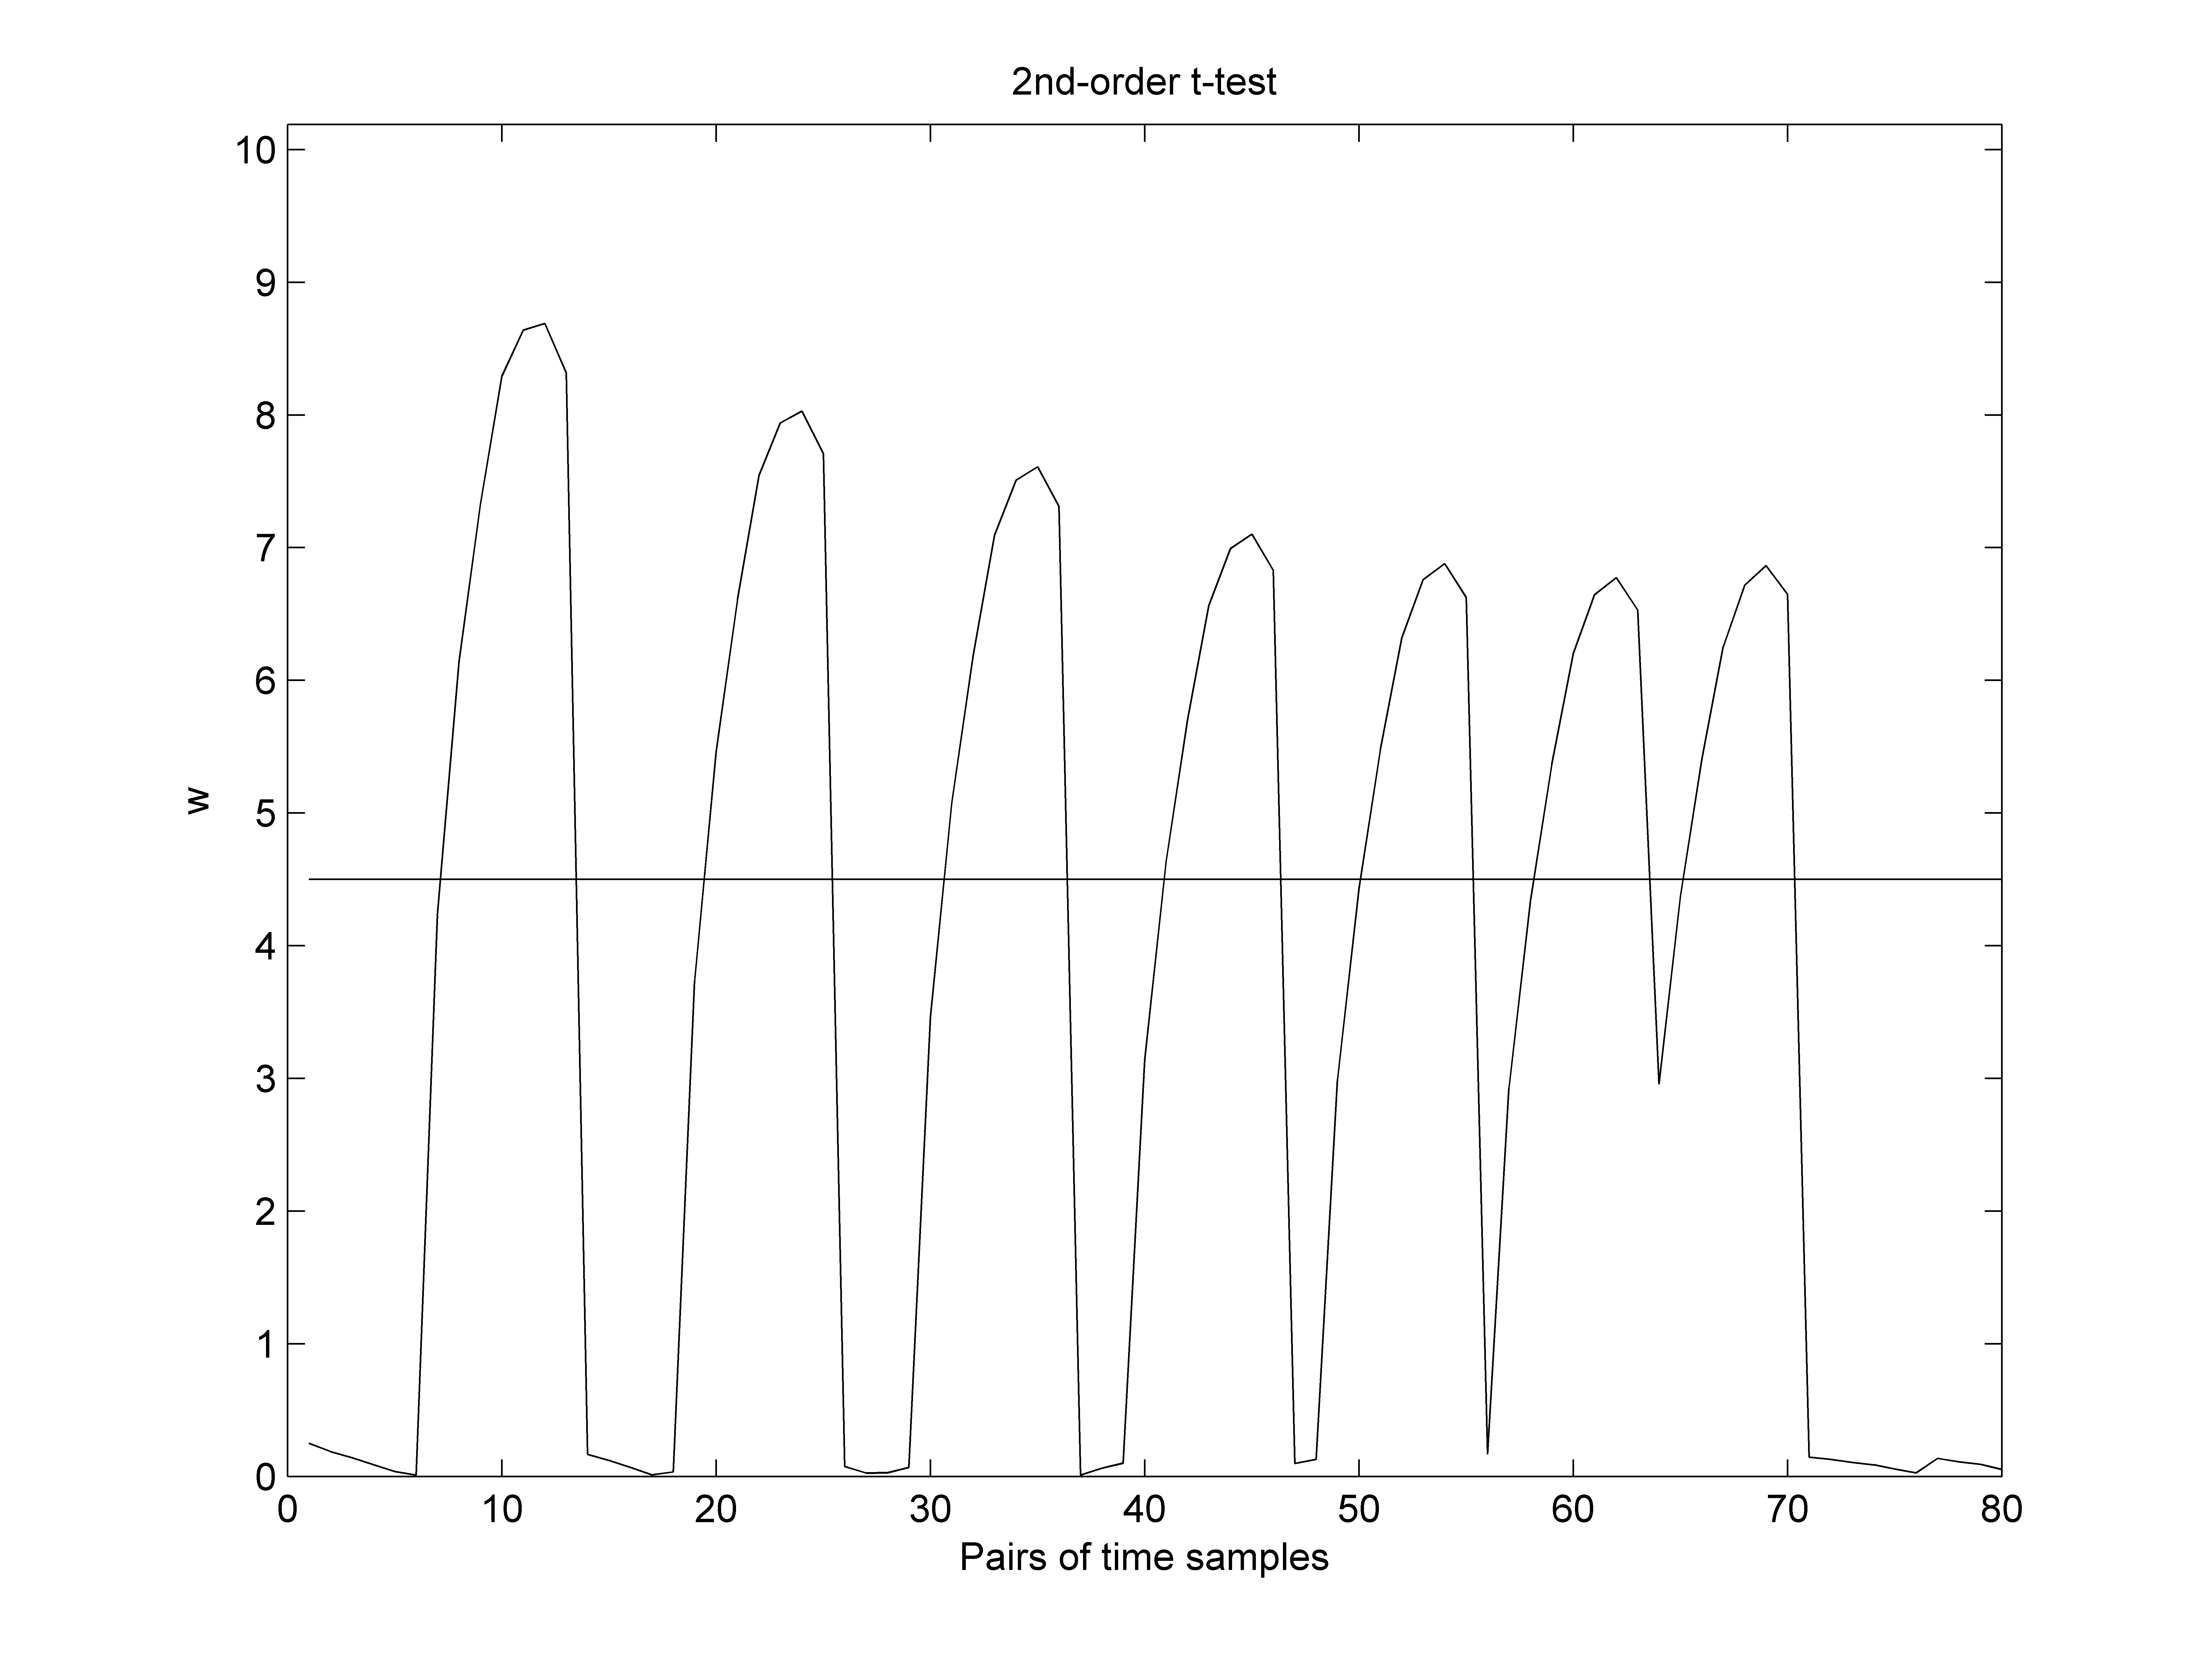
\includegraphics[width=\textwidth]{{fig/t_order2.png}}

        \caption{\scriptsize{Consevative hardened Sbox, 2nd-order t-test, 25k random vs. 25k fixed.}}
\label{t_order2}
    \end{subfigure} \hspace{15px}
 \begin{subfigure}[b]{0.40\textwidth}
        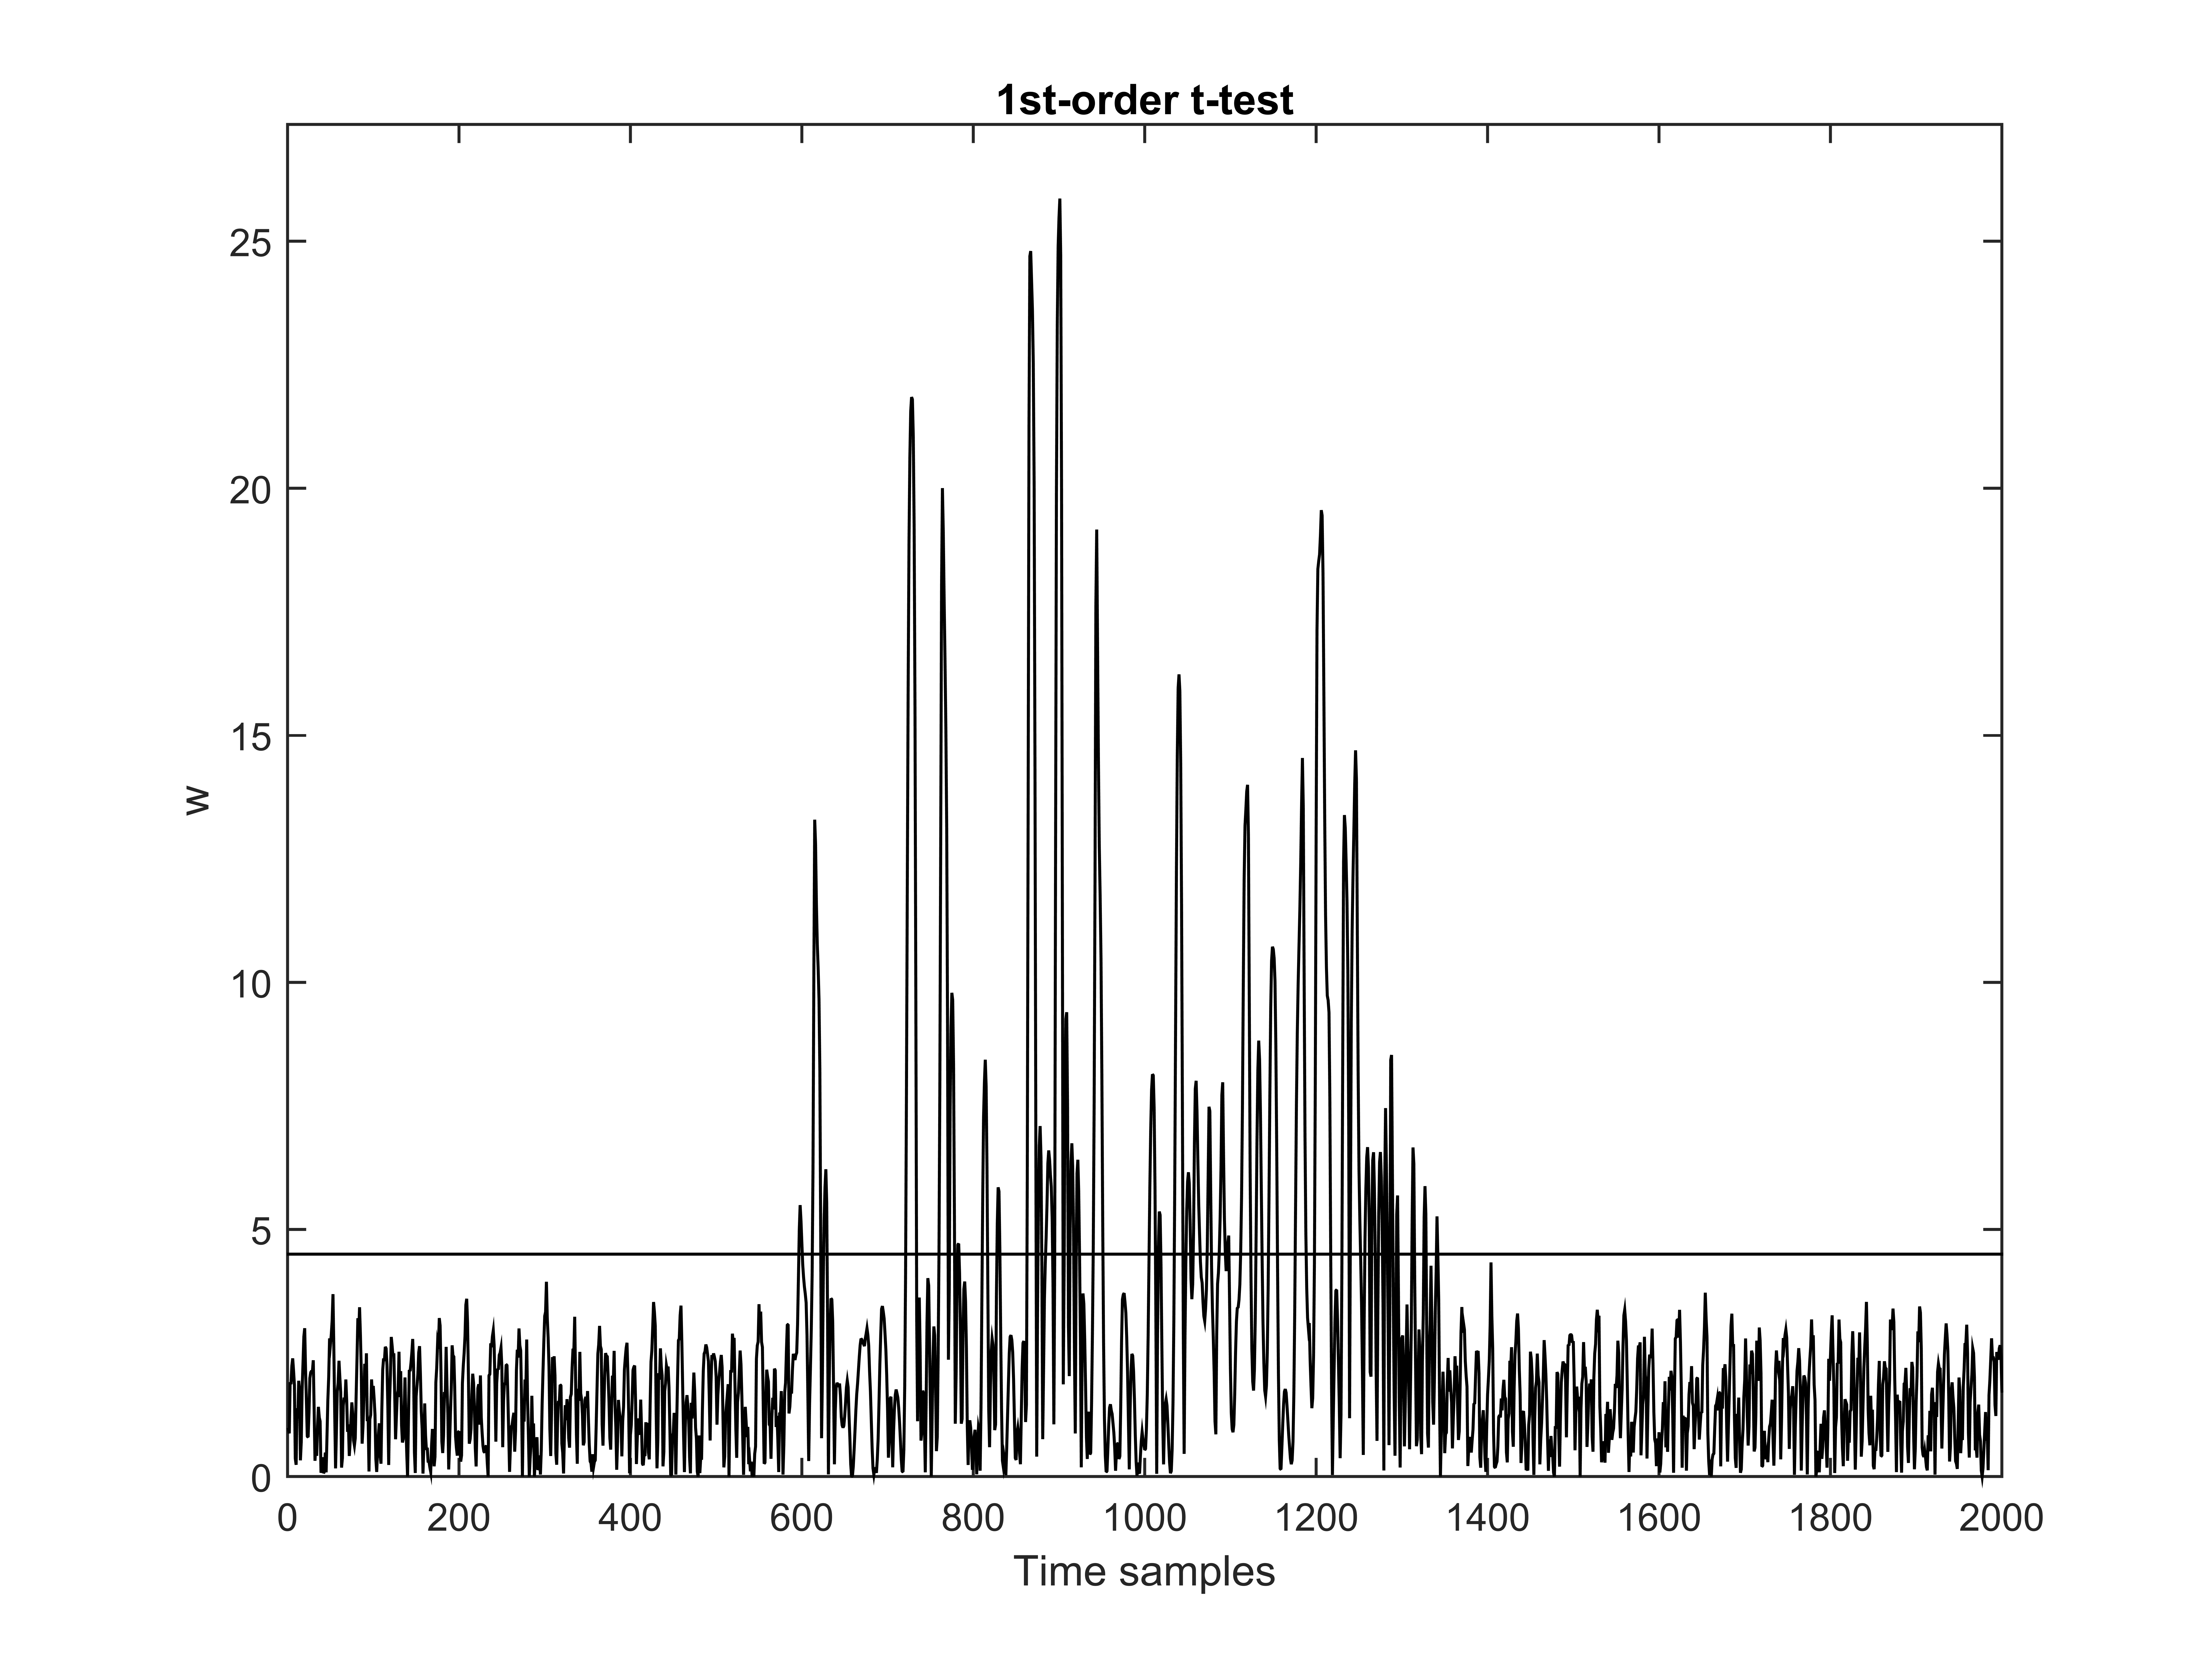
\includegraphics[width=\textwidth]{{fig/softbox.png}}

        \caption{\scriptsize{Naive Sbox, 1st-order t-test, 1k random vs. 1k fixed.}}
\label{softbox}
    \end{subfigure}

   
    \caption{Hardened and naive Sbox evaluations}\label{fig:sboxleak}
\end{figure}
So far, the only way to guarantee the actual security order of a real-world implementation was to increase the scheme's theoretical order $d$, in order to ensure that the implementation attains an actual order of $\lfloor \frac{d}{2} \rfloor$~\cite{DBLP:conf/cardis/BalaschGGRS14, DBLP:journals/iacr/GrootPPSB16}. Clearing the ILA-breaching effects requires a significant overhead and is device-dependent, yet it is the only technique known to us that can enforce 1st-order, univariate security. In addition, hardening does not increase the scheme order $d$, thus the random number generation (RNG) cost is not increased. The previous suggestions require a higher scheme order, hence a significant overhead, since both the implementation cost and the RNG cost are quadratic w.r.t. the order. We compare the ``hardened" 1st-order and ``naive" 2nd-order implementation costs (in clock cycles) and we observe that hardening the 1st-order Sbox is slower than increasing the scheme's order from 1 to 2 (both in the efficient and in the conservative case). Still, the solution requires no extra RNG and we maintain that removing these effects can also be beneficial to higher-order implementations, i.e. it is complimentary to masking. The extent to which higher-order implementations can benefit from removing such effects remains an open problem.


















